%!TEX root = ../main.tex
%-------------------------------------------------------------------------------
\section{Example}\label{Example}
%-------------------------------------------------------------------------------
We now analyze a canonical EKW model. We start with an outline and discussion of the occupational choice model presented in \citet{Keane.1994}. The model is deliberately simple, but already contains the core components required for serious research applications. We will parameterize it so that we can simulate a data set that mirrors the basic patterns often documented in actual data on observed individual decisions. We conclude by sketching its specification, simulation, and calibration using our group's research codes \verb+respy+ and \verb+estimagic+.
%-------------------------------------------------------------------------------
\subsection{Keane \& Wolpin (1994)}
%-------------------------------------------------------------------------------
We study individuals over their working life for $T = 40$ years from age 16 to 65. Individuals can choose to either work in one of two occupations ($a_t = 1, 2$), attend school ($a_t = 3$), or stay at home ($a_t = 4$). Immediate rewards are determined as follows:
%
\begin{align*}
r_t(s_t, a_t) = \begin{cases} w_{1t} =
\exp\{\alpha_{10} + \alpha_{11}g_t + \alpha_{12}e_{1t} + \alpha_{13}e^2_{1t} + \alpha_{14}e_{2t} + \alpha_{15}e^2_{2t} + \epsilon_{1t}\} & \text{if}\; a_t = 1 \\
w_{2t} = \exp\{\alpha_{20} + \alpha_{21}g_t + \alpha_{22}e_{1t} + \alpha_{23}e^2_{1t} + \alpha_{24}e_{2t} + \alpha_{25}e^2_{2t} + \epsilon_{2t}\}& \text{if}\; a_t = 2 \\
\beta_0 - \beta_1 \Ind[\,g_t \geq 12\,] - \beta_2\Ind[\,a_{t - 1} \neq 3\,] + \epsilon_{3t}& \text{if}\; a_t = 3 \\
\gamma_0 + \epsilon_{4t}& \text{if}\; a_t = 4. \\
\end{cases}
\end{align*}
%
$g_t$ is the number of periods of schooling obtained by the beginning of period $t$, $e_{1t}$ and $e_{2t}$ are the number of periods that the individual worked in the two occupations respectively. The reward for each labor market alternative corresponds to its wage $(w_{1t}, w_{2t})$ and $\alpha_{1}$ and $\alpha_{2}$ are thus parameters associated with the wage functions. They capture the returns to schooling and occupation-specific human capital. Turning to the rewards from school attendance, $\beta_0$ is the consumption reward of schooling, $\beta_1$ is the post-secondary cost of schooling, and $\beta_2$ is an adjustment cost associated with returning to school after dropping out. The mean reward of the home alternative is denoted $\gamma_0$. The $\epsilon_{at}$'s are alternative-specific shocks to occupational productivity, the consumption value of schooling, and home time.\\

\noindent Given the structure of the reward functions and imposing that the shocks are not correlated across time, the state at time $t$ is $s_t = \{g_t,e_{1t},e_{2t},a_{t - 1},\epsilon_{1t},\epsilon_{2t},\epsilon_{3t},\epsilon_{4t}\}$.
%
The current stock of human capital is observable $\{g_t,e_{1t},e_{2t},a_{t - 1}\}$ to the individual and the economist. It evolves deterministically according to the following rules:
%
\begin{align*}
    e_{1,t+1} &= e_{1t} + \Ind[\,a_t = 1\,] \\
    e_{2,t+1} &= e_{2t} + \Ind[\,a_t = 2\,] \\
    g_{t+1}   &= g_{t\phantom{2}}    +  \Ind[\,a_t = 3\,].
\end{align*}

\noindent The shocks $\{\epsilon_{1t},\epsilon_{2t},\epsilon_{3t},\epsilon_{4t}\}$ are only observable by the individual and evolve stochastically according to a joint normal distribution.\\

\noindent \citet{Keane.1994} analyze three different parameterizations of the model, and we reproduce the second one for this example. Initially, individuals are identical and have no labor market experience $(e_{11} = e_{21} = 0)$ but ten years of schooling $(g_1 = 10)$. Different choices over the life cycle are then simply the cumulative effects of different shocks.\\

\noindent One year of additional schooling increases wages by only 4\% in the first occupation compared to 8\% in the second. We will thus refer to the former as blue-collar and the latter as white-collar going forward. Starting wages are considerably lower in the white-collar sector, but wages increase more rapidly with occupation-specific experience compared to blue-collar wages. Own-work experience is highly valuable in both occupations. However, while white-collar wages increase with blue-collar experience as well, the opposite is not true. There is a consumption value of schooling of \$5,000, but the total cost of pursuing post-secondary education is considerable and amounts to \$5,000. Once leaving school, individuals incur a nearly prohibitive cost of \$15,000 for re-enrolling. Individuals are forward-looking with a discount factor $\delta$ of 0.95.\\

\noindent We simulate the life cycle histories of 1,000 individuals. Figure \ref{Choices over the life cycle} shows the share of individuals choosing each of the four alternatives by period. Initially, roughly 60\% of individuals enroll in school, but this share declines rapidly, and only 19\% attain any post-secondary education. Right away, about 30\% of individuals are working in the blue-collar occupation.  Blue-collar employment initially increases even further to peak at 65\% as individuals are leaving school and entering the labor market. White-collar employment steadily rises over the life cycle but never reaches more than 40\%. About 5\% of individuals stay at home each period.

\begin{figure}[ht!]\centering
\caption{Choices over the life cycle}\label{Choices over the life cycle}
\scalebox{0.35}{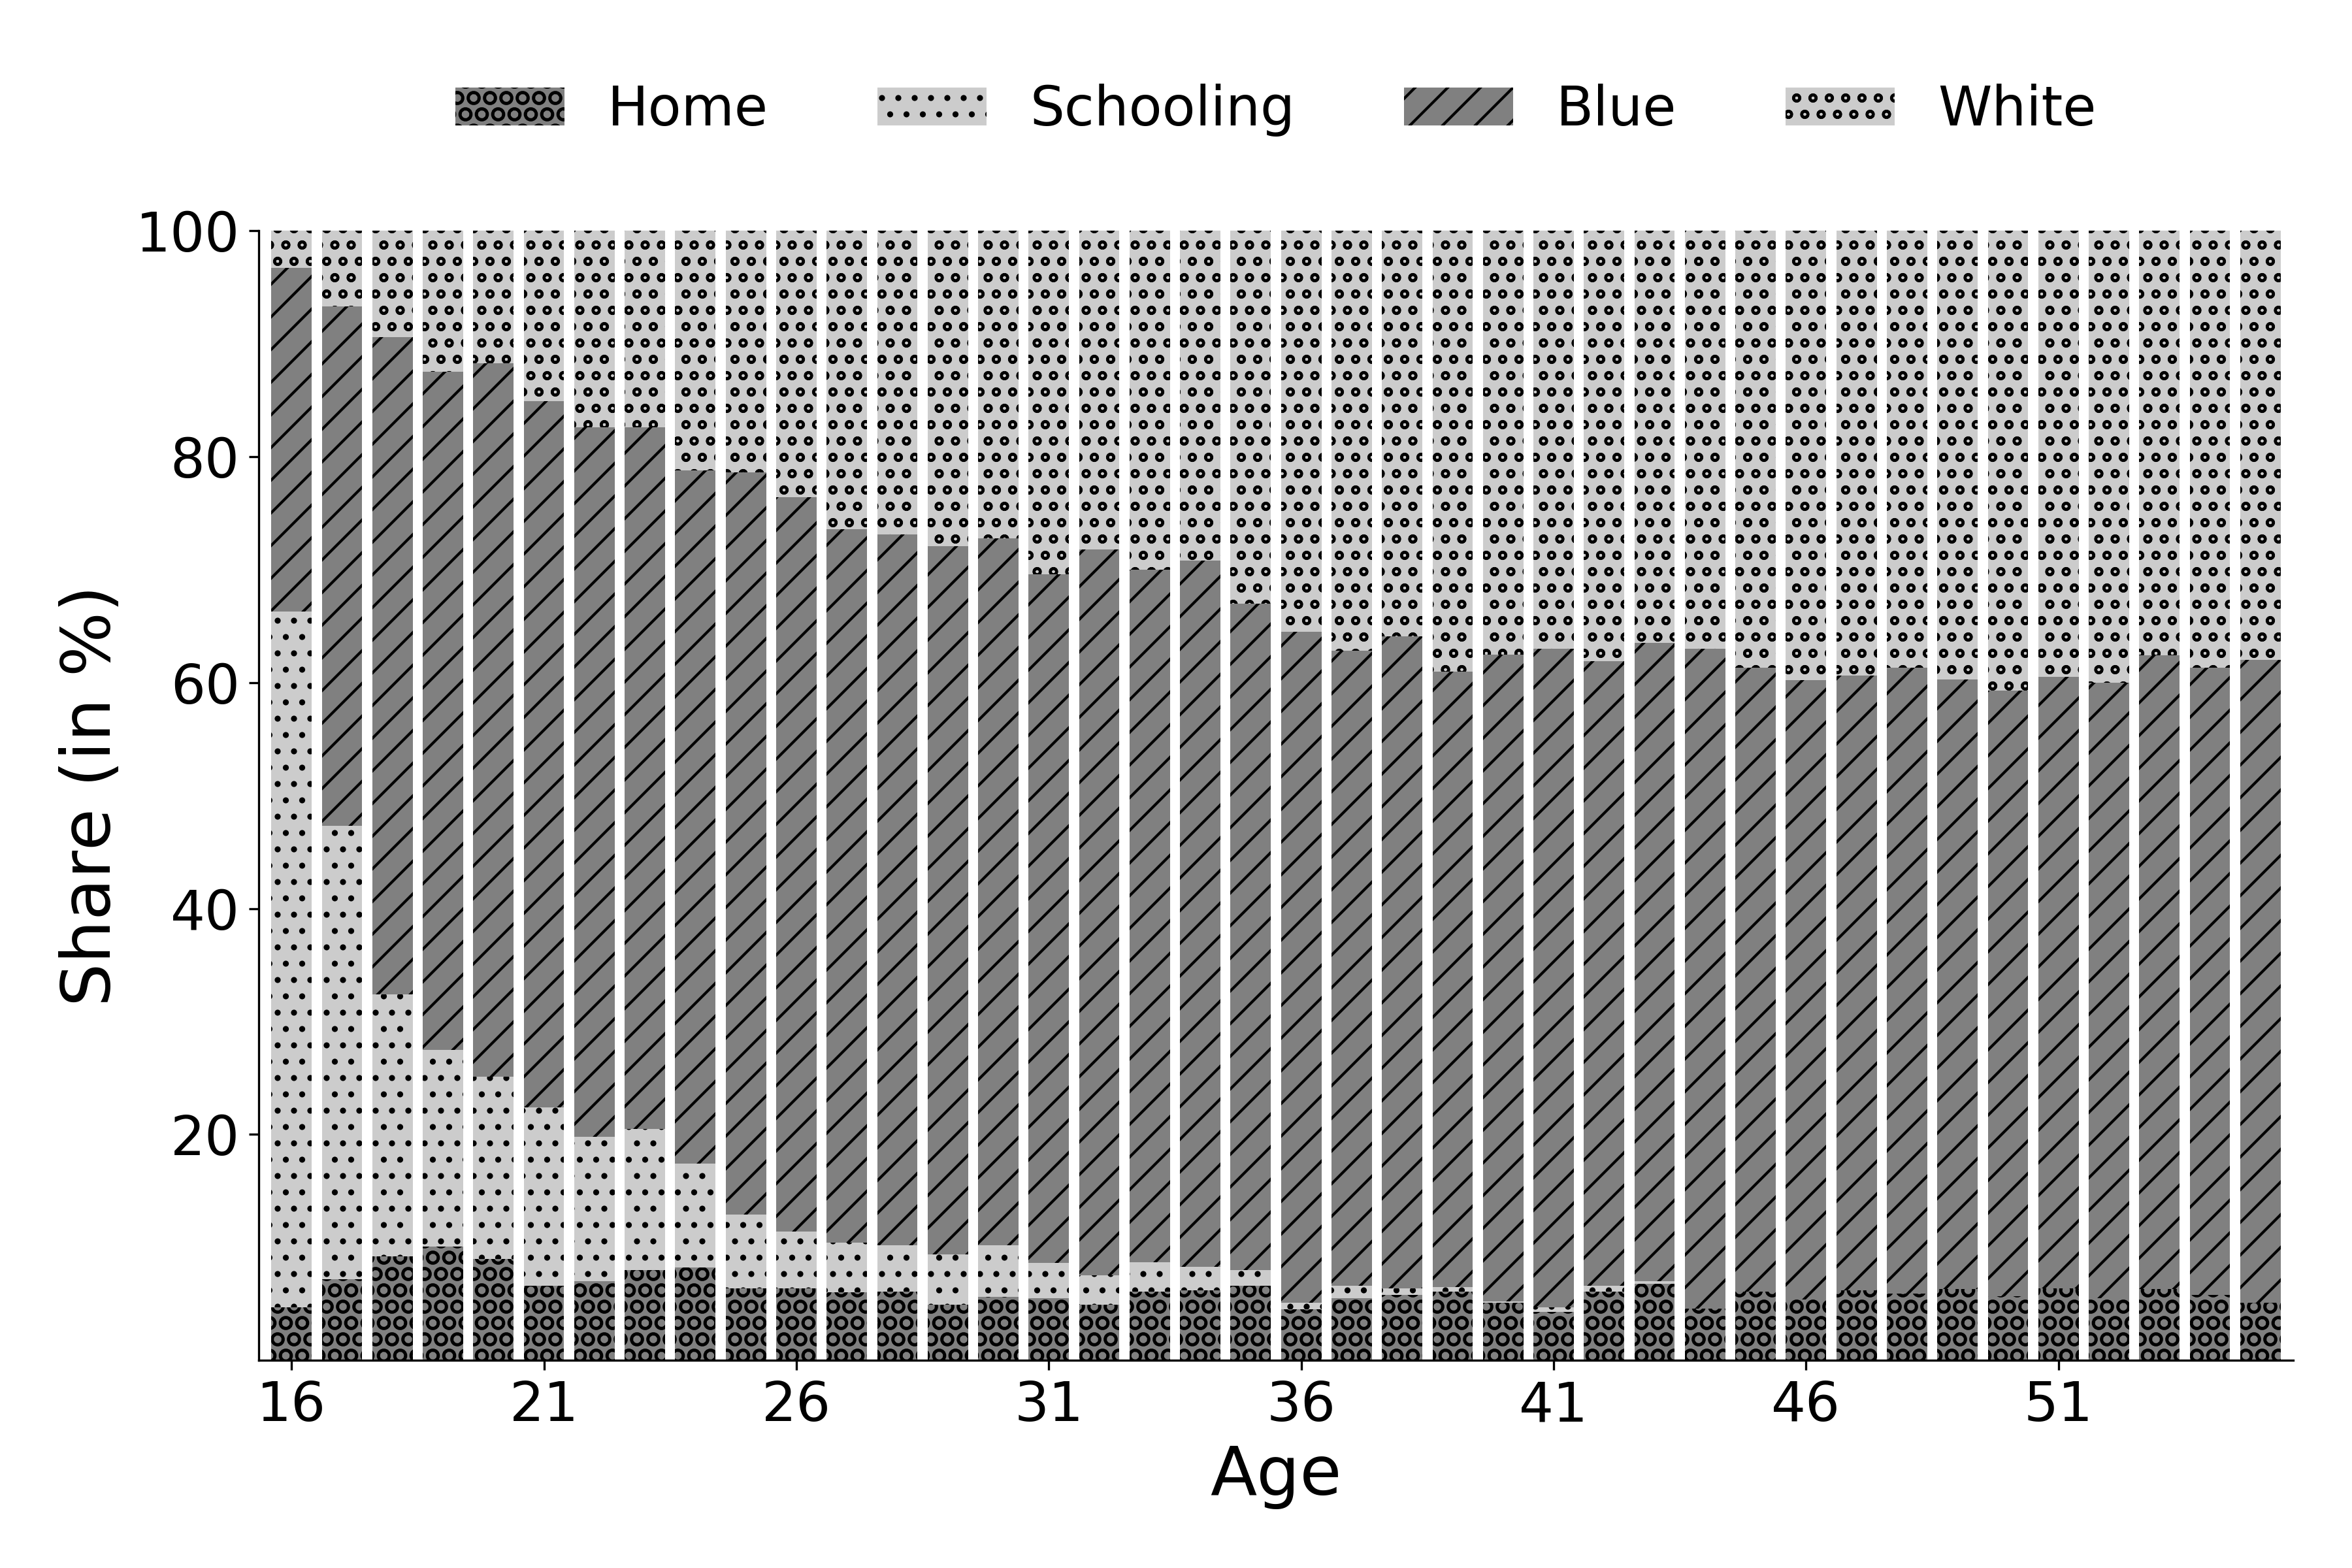
\includegraphics{fig-observed-choices-black-white}}
\end{figure}\FloatBarrier

\noindent Overall, average final schooling is slightly above a high school degree with 12.5 years. Individuals choose to incur the immediate costs of their schooling investments in the form of tuition and foregone wages right at the start. Doing so maximizes their ability to reap the reward of increased wages over the remaining time periods.\\

\noindent Figure \ref{Economic mechanism and policy forecast} illustrates the ability of the model to quantify the impact of economic mechanisms and to forecast the effect of public policies. On the left, we vary the discount factor capturing time preferences between $0.945$ and $0.955$ while we reduce $\beta_1$ by the size of a tuition subsidy of up to $\$1,500$ on the right. In both cases, we are interested in the changes to average final schooling.

\begin{figure}[h!]\centering
\caption{Economic mechanism and policy forecast}\label{Economic mechanism and policy forecast}
\subfloat[Time preference]{\scalebox{0.25}{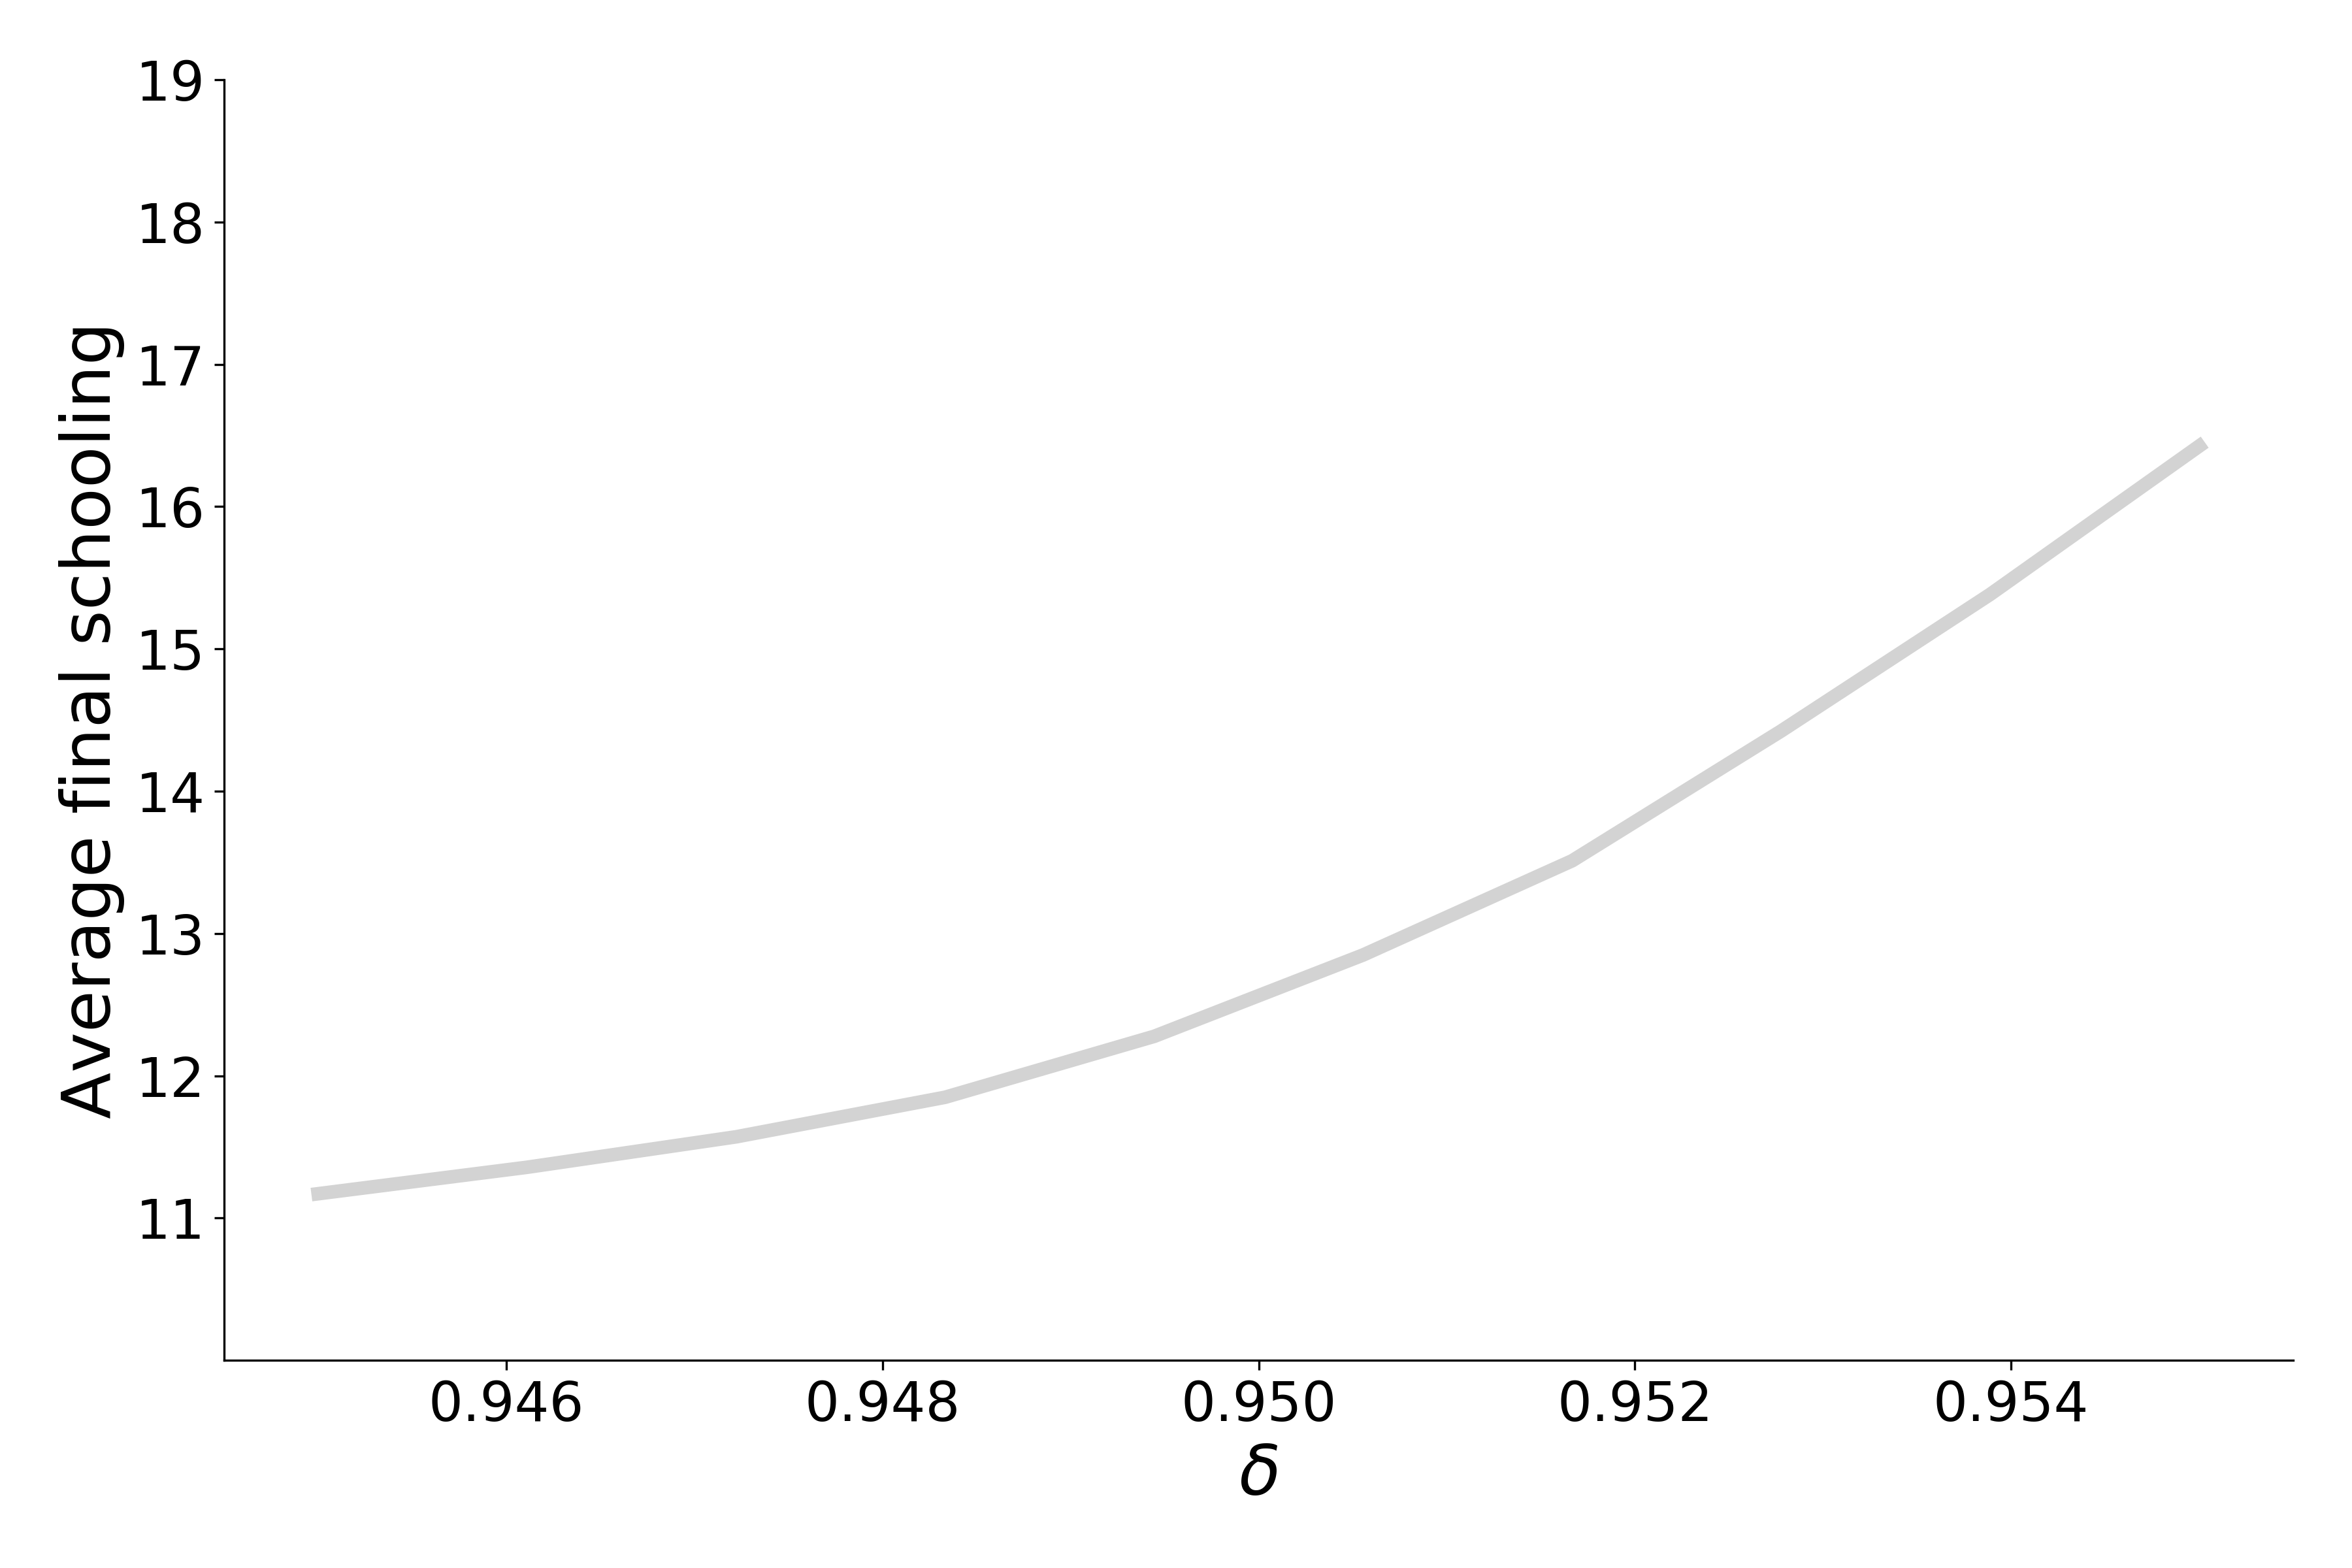
\includegraphics{fig-economic-mechanisms-black-white}}}\hspace{0.3cm}
\subfloat[Tuition subsidy]{\scalebox{0.25}{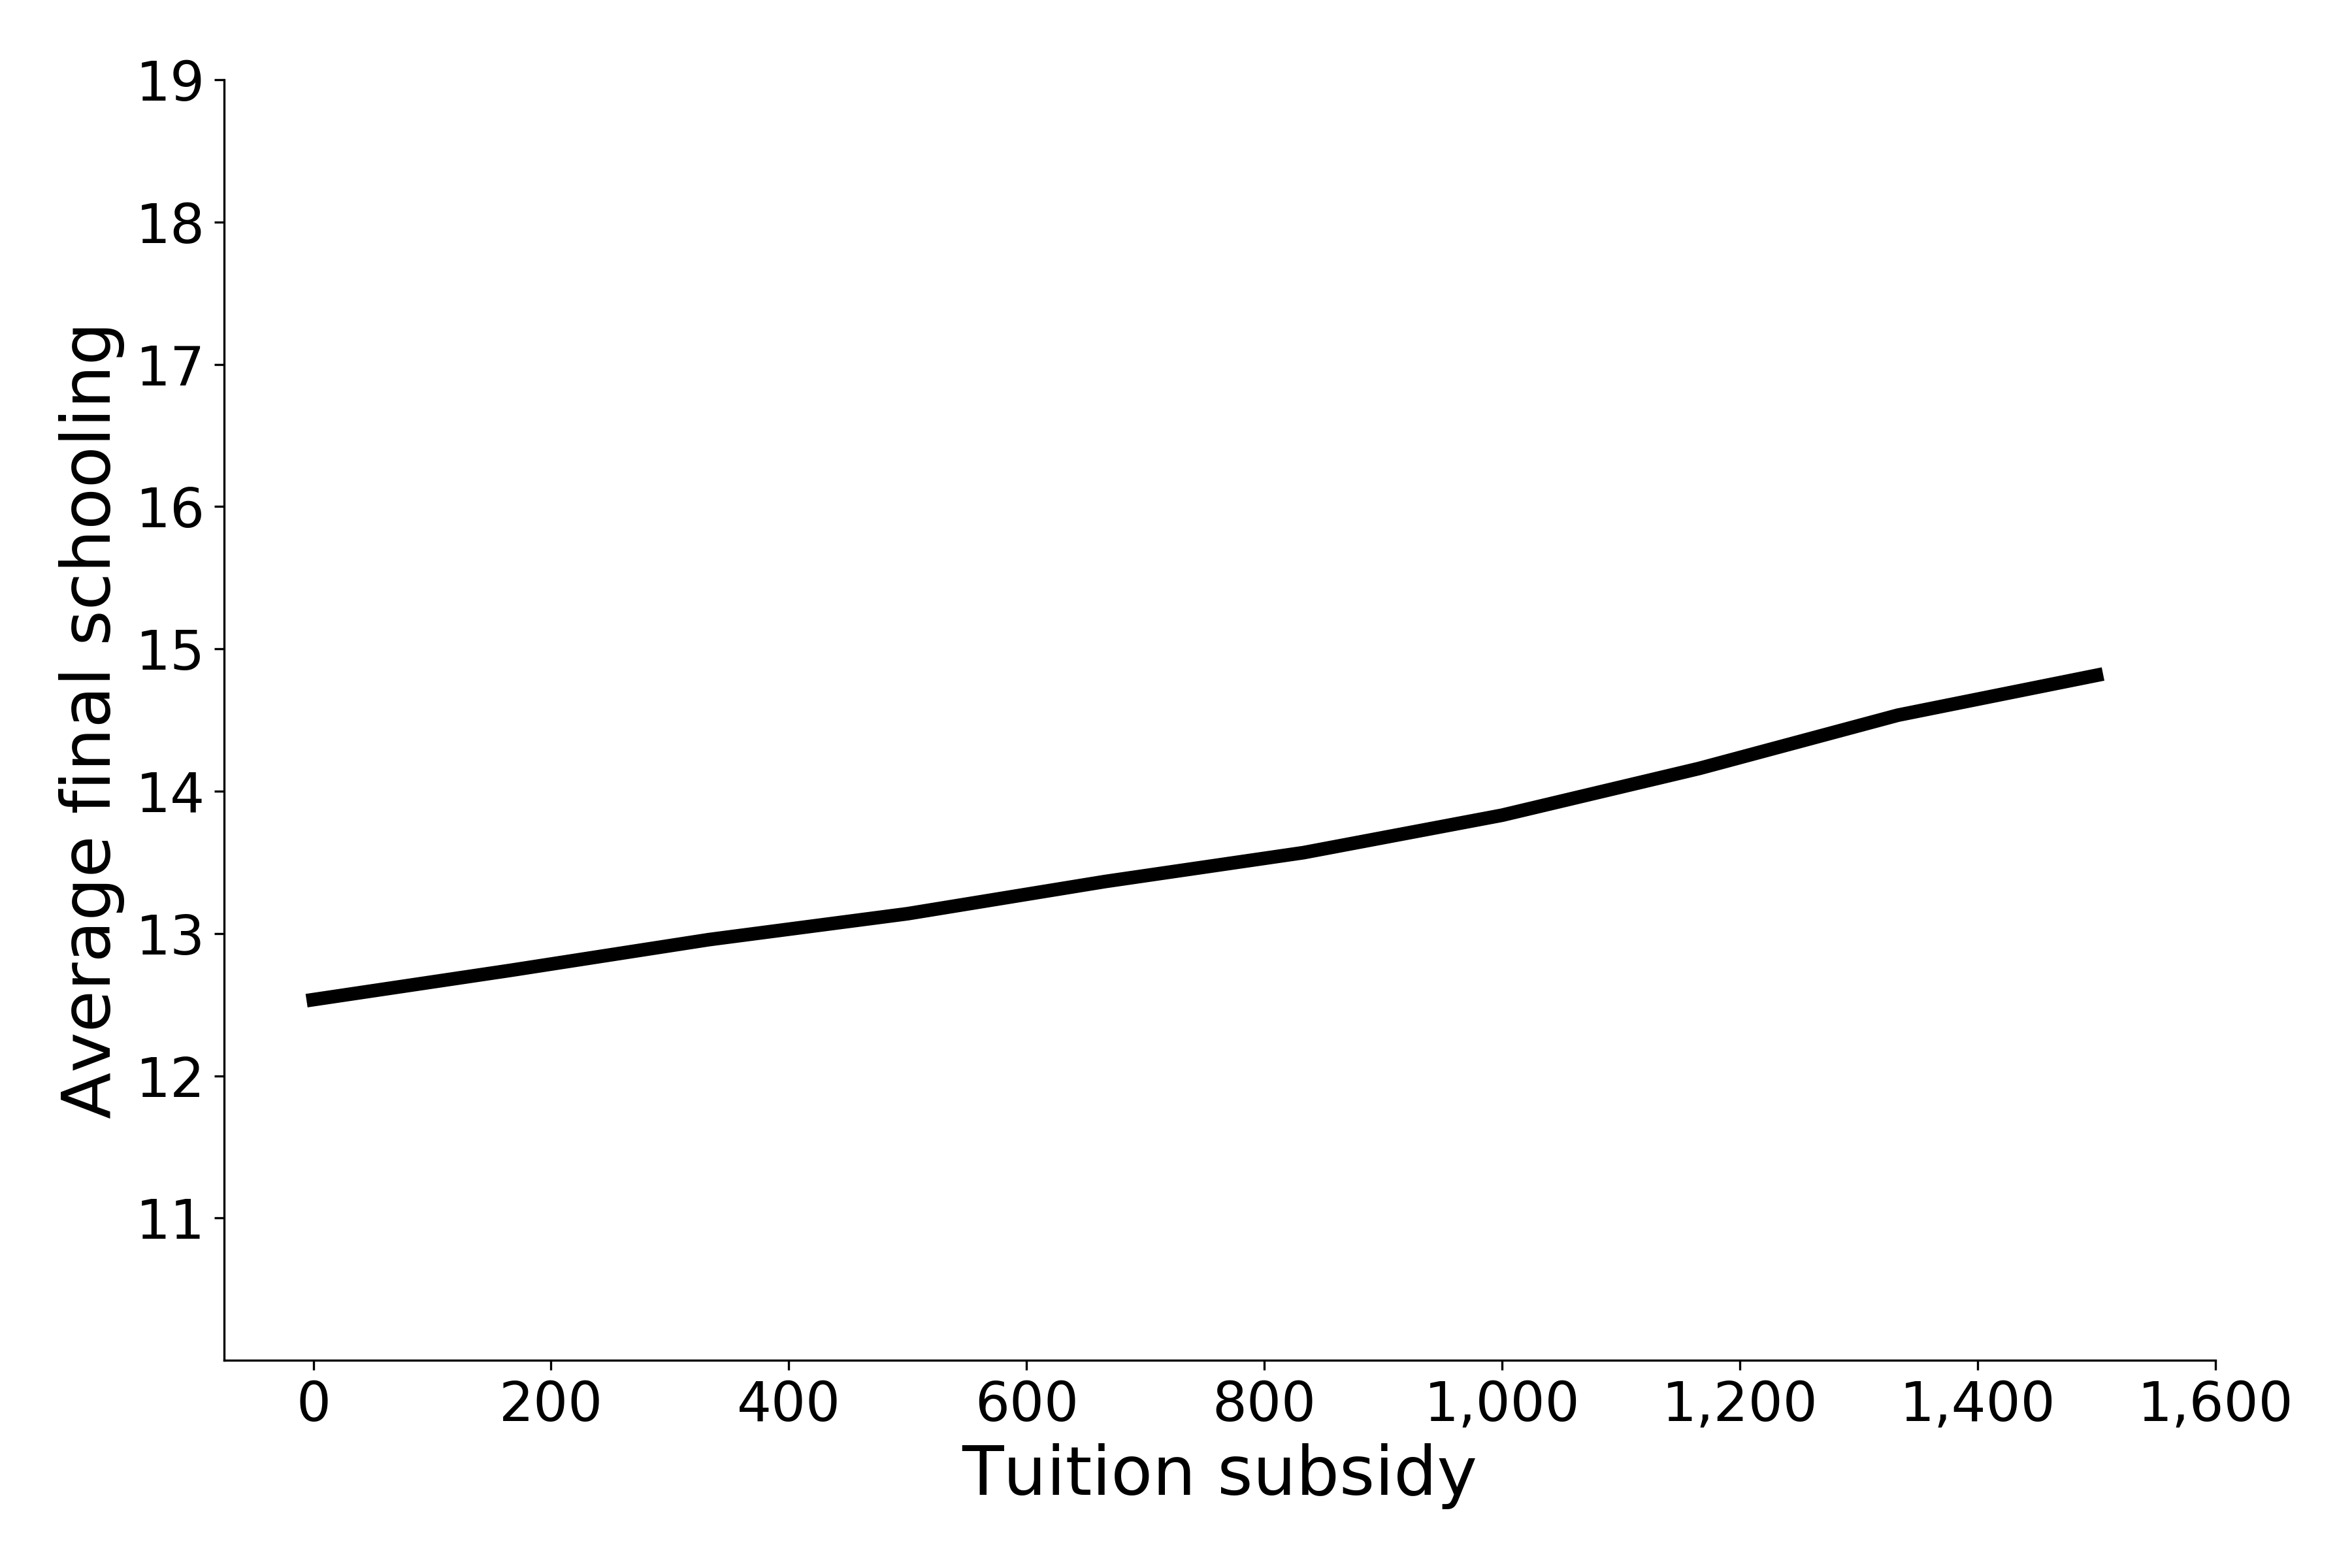
\includegraphics{fig-policy-forecast-black-white}}}
\end{figure}\FloatBarrier

\noindent Increases in the discount factor and the tuition subsidy both result in higher average final schooling. However, they do so for very different reasons. While individuals put more emphasis on the future benefits of their schooling investment in the former, they react to a reduction of its immediate cost in the latter.
%-------------------------------------------------------------------------------
\subsection{\texttt{respy} and \texttt{estimagic}}
%-------------------------------------------------------------------------------
Our research group is actively developing two research codes that allow analyzing EKW models. \verb+respy+ allows for their flexible specification and simulation, and \verb+estimagic+ provides the infrastructure for their calibration. We briefly showcase the typical workflow of using both packages in our research.\\

\noindent Figure \ref{Typical workflow} illustrates a typical workflow. Initially, the user provides the observed data, the parameterization of the model, and other options to \verb+respy+. All together define the structure of the model, and we can construct the functionality for the simulation of data and the evaluation of the criterion function. \verb+estimagic+ allows calibrating the model to the observed data. The results from the calibration steps are used to, for example, analyze the economic mechanisms underlying the observed behaviors.

\begin{figure}[ht!]\centering
\caption{Typical workflow}\label{Typical workflow}
\lstset{language=python, morekeywords={as}, ndkeywords={=}, ndkeywordstyle=\color{black}, keywordstyle=\color{black}, commentstyle=\color{black}, emph={}, emphstyle=\color{violet}, basicstyle=\footnotesize, frame=lines,   showlines=true}
\lstinputlisting{../material/workflow.py}
\end{figure}\FloatBarrier

\noindent Figure \ref{Model specification} shows the model specification files for \citet{Keane.1994}. The file on the left sets the parameter values for the reward functions and the distribution of the unobservable state variables. On the right, we provide details on the construction of the observed state variables and numerous tuning parameters for the numerical solution of the model.

\begin{figure}[h!]\centering
\caption{Model specification}\label{Model specification}
\subfloat[Parameterization]{\scalebox{0.25}{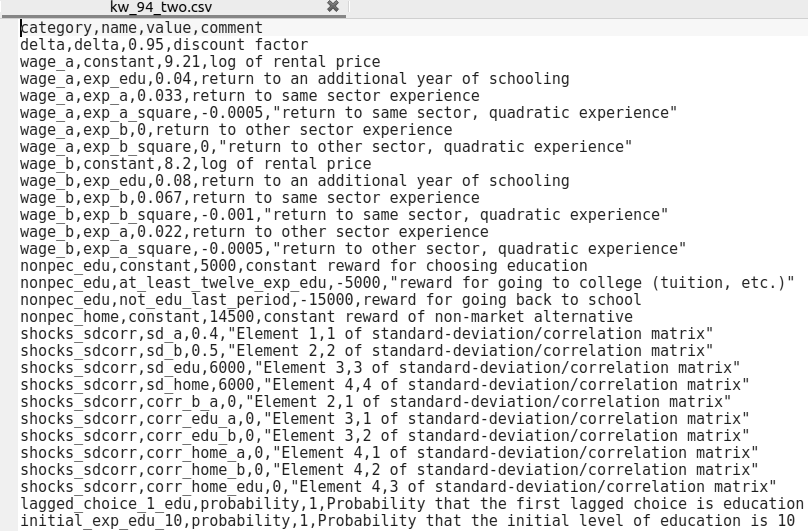
\includegraphics{crop-params-black-white}}}\hspace{0.3cm}
\subfloat[Options]{\scalebox{0.25}{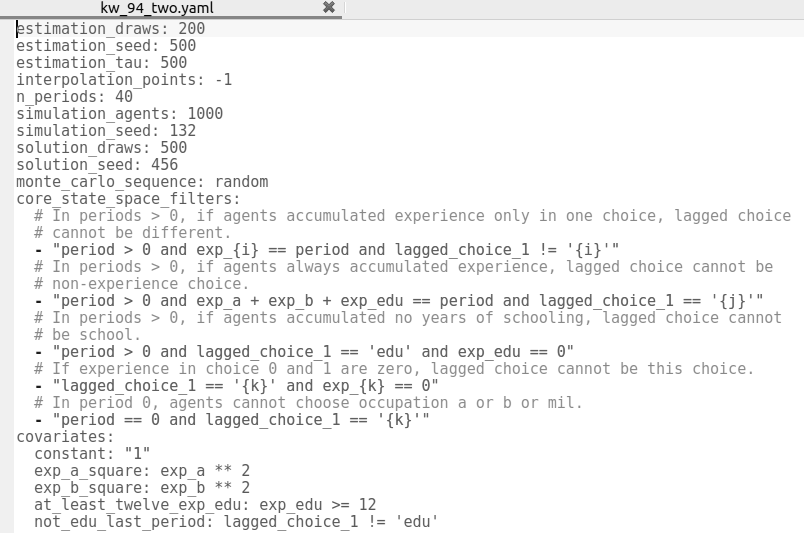
\includegraphics{crop-options-black-white}}}
\end{figure}\FloatBarrier

\noindent Figure \ref{Dashboard} depicts the dashboard provided by \verb+estimagic+ to monitor the progress and parameter values of the calibration in real-time. This allows us to detect problems during calibration right away and facilitates the debugging process.

\begin{figure}[h!]\centering
\caption{Dashboard}\label{Dashboard}
\scalebox{0.50}{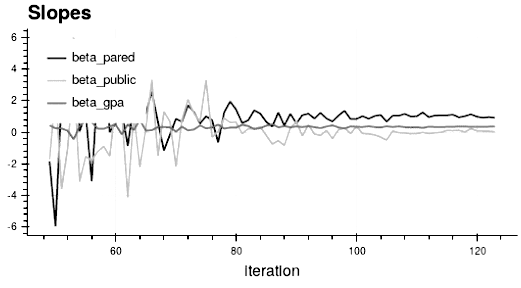
\includegraphics{crop-dashboard-black-white}}
\end{figure}\FloatBarrier

\noindent We adopt a modern software engineering workflow in the development of both packages and tutorials, source code, testing harness, as well as implementation details are available in their respective online documentations at \url{https://respy.readthedocs.io} and \url{https://estimagic.readthedocs.io}.
